\documentclass{article} % say
\usepackage{tikz}
\begin{document}
We are working on

\vspace{1cm}

\begin{tikzpicture}
  \draw (-1.5,0) -- (1.5,0);
  \draw (0,-1.5) -- (0,1.5);
\end{tikzpicture}.

\vspace{1cm}

\begin{tikzpicture}
  \draw (-1.5,0) -- (1.5,0);
  \draw (0,-1.5) -- (0,1.5);
  \draw (-1,0) .. controls (-1,0.555) and (-0.555,1) .. (0,1)
               .. controls (0.555,1) and (1,0.555) .. (1,0);
\end{tikzpicture}

\vspace{1cm}

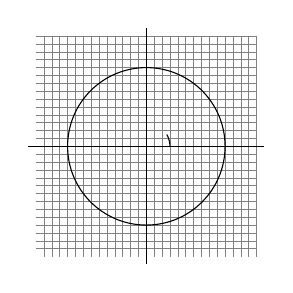
\begin{tikzpicture}
  \draw[step=.1cm,gray,very thin] (-1.4,-1.4) grid (1.4,1.4);
  \draw (-1.5,0) -- (1.5,0);
  \draw (0,-1.5) -- (0,1.5);
  \draw (0,0) circle (1cm);
  \draw (3mm,0mm) arc (0:30:3mm);
\end{tikzpicture}

\vspace{1cm}

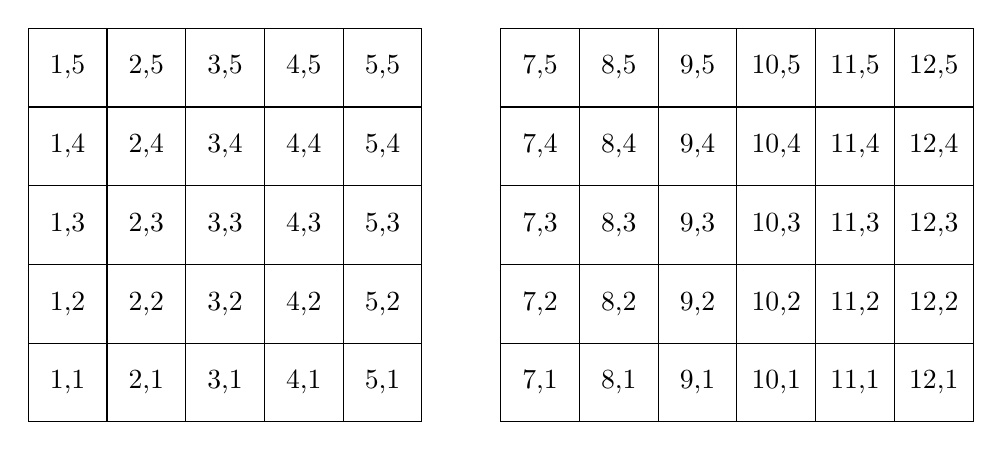
\begin{tikzpicture}
  \foreach \x in {1,2,...,5,7,8,...,12}
    \foreach \y in {1,...,5}
    {
      \draw (\x,\y) +(-.5,-.5) rectangle ++(.5,.5);
      \draw (\x,\y) node{\x,\y};
    }
\end{tikzpicture}

\vspace{1cm}


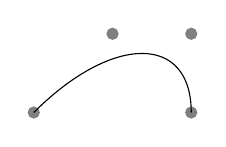
\begin{tikzpicture}
  \filldraw [gray] (0,0) circle (2pt)
                    (1,1) circle (2pt)
                    (2,1) circle (2pt)
                    (2,0) circle (2pt);
  \draw (0,0) .. controls (1,1) and (2,1) .. (2,0);
\end{tikzpicture}

\vspace{1cm}
\begin{tikzpicture}
	[kashyap/.style={help lines,color=blue!50}]
	\draw[kashyap, rotate=30] (0,0) ellipse (30mm and 15mm);
	\draw[kashyap] (3,3) ellipse (30mm and 15mm);
\end{tikzpicture}


\end{document}

